%%%%%%%%%%% INFORMAÇÕES BÁSICAS %%%%%%%%%%%%%%%%%%%%%
% Versão: 		1.0
% Autor:		Rodrigo Guimarães
% Finalidade:	Descritivo do SPT para o Trabalho 2
%				da disciplina SI 2016.2
%%%%%%%%%%% FIM INFORMAÇÕES BÁSICAS %%%%%%%%%%%%%%%%


%%%%%%%%%%% INCLUSÃO DE PACOTES %%%%%%%%%%%%%%%%
% Classe Base do Documento: Artigo
\documentclass [12pt]{article}
% Layout do Papel
\usepackage{../../Layout/Layout_Documento}
% Case não funcione, verificar o diretório do arquivo 'Layout_Documento.sty'
%\usepackage{lipsum}
%%%%%%%%%%% FIM INCLUSÃO DE PACOTES %%%%%%%%%%%

%%%%%%%%%%% INFORMAÇÕES BÁSICAS %%%%%%%%%%%%%%%
\title {Modelagem}
\subtitle {DER}
\date {\today}
%%%%%%%%%%% FIM INFORMAÇÕES BÁSICAS %%%%%%%%%%%

%%%%%%%%%%% DOCUMENTO %%%%%%%%%%%%%%%%%%%%%%%%%
\begin{document}
	\inserirTitulo

	Para a modelagem do DER (Diagrama Entidade Relacionamento) foi utilizado o~\textit{software}~\textbf{MySQL Workbench}\footnote{\textit{MySQL Workbench}, https://www.mysql.com/products/workbench/}, por ser uma ferramenta já utilizada para modelagem na disciplina~\textit{Bando de Dados}, tendo como resultado a Figura~\ref{fig:modeloDER}.
	
	Por conta da ferramenta, o modelo de DER desenvolvido está baseado na modelagem padrão desenvolvida por James Martin, demonstrada na Figura~\ref{fig:exmodeloDER}. Além disso, há um informações referentes ao Modelo Relacional (MR), como: as chaves primárias e segundárias do que virião a ser as tabelas, propriamente ditas, no Banco de Dados; por isso, tais informações não foram retiradas da modelagem.

	\begin{figure}[h]
		\centering
		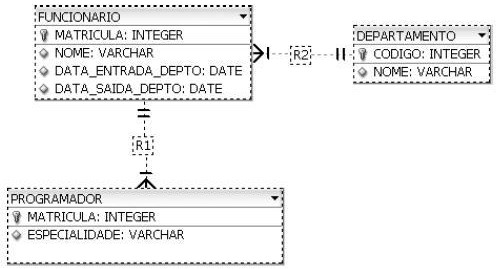
\includegraphics[width=.68\textwidth]{modelagem_JamesMartin}
		\caption{Exemplo de modelagem DER, por James Martin.}
		\label{fig:exmodeloDER}
	\end{figure}

	\begin{figure}[h]
		\centering
		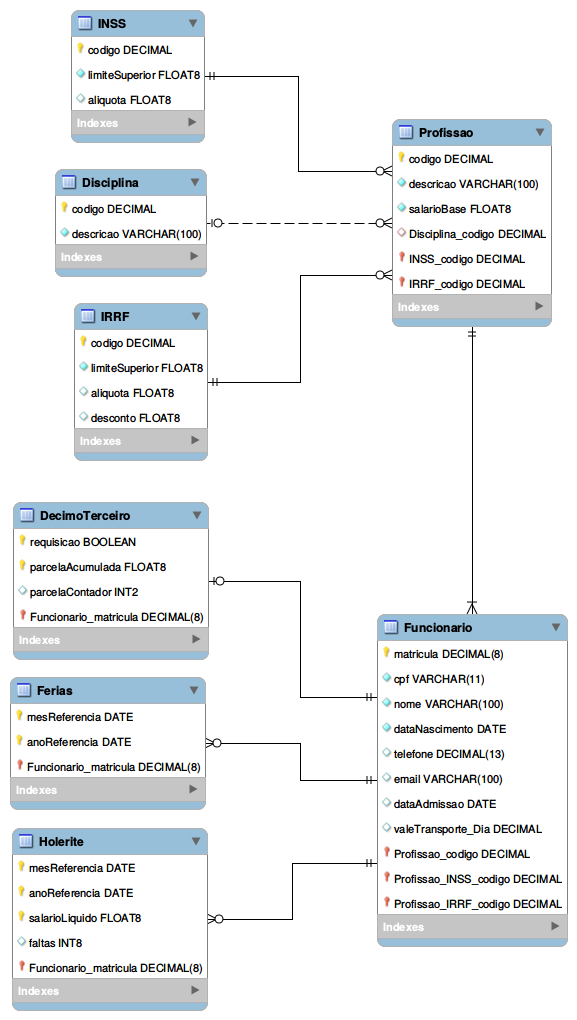
\includegraphics[width=.68\textwidth]{Modelagem_DER_3}
		\caption{Modelo DER gerado.}
		\label{fig:modeloDER}
	\end{figure}
	
\end{document}
%%%%%%%%%%% FIM DOCUMENTO %%%%%%%%%%%%%%%%%%%%%
